\newpage

\begin{usecase}
  \addheading{Use-Case Description}
  \addsingletwocolumnrow{Name}{oeRequestEMSAssistance}
  \addsingletwocolumnrow{Scope}{System}
  \addsingletwocolumnrow{Altitude}{subfunction}
   
  \addrowheading{Parameters}
  \addnumberedsinglerow{}{\msrcode{Message:dtComment} - A message from the \msrcode{actCoordinator} to the \msrcode{actEMS}}
  \addnumberedsinglerow{}{\msrcode{UniqueIDOftheReq:dtRequestID} - a request
  identification enabling\msrcode{actCoordinator}s and \msrcode{actEMS}s to differentiate requests.}
  \addnumberedsinglerow{}{\msrcode{NumberofVehiculesin
  accident:dtNbrofVehiculesInAccident} - the number of vehicles involved in the accident.}
  \addnumberedsinglerow{}{\msrcode{NumberofVictimsinaccident:dtNbrofVictims} -
  the number of victims involved in the accident.}
  \addnumberedsinglerow{}{\msrcode{TypeOfreqEMSAssistance:ctEMSType} - the type
  of EMS unit requested.(RequestFireFighter, RequestPolice and RequestAmbulance)You can ether request one of each or just two or all.}
  
  \addrowheading{Primary actor(s)}
  \addnumberedsinglerow{}{\msrcode{Coordinator[active]}}
  
  \addrowheading{Secondary actor(s)}
  \addnumberedsinglerow{}{None.}
  
  \addrowheading{Goal(s) description}
  \addsinglerow{the \msrcode{actCoordinator}'s goal is to request a EMS unit to provide assistance to the victims of a car accident.}
  
  \addrowheading{Reuse}
  \addnumberedsinglerow{}{none}

  \addrowheading{Protocol condition(s)}
  \addnumberedsinglerow{}{the \msricrash system has been deployed.}
  \addnumberedsinglerow{}{an Alert has been received by our system.}
  
  \addrowheading{Pre-condition(s)}
  \addnumberedsinglerow{}{none}
  
  \addrowheading{Main post-condition(s)}
  \addnumberedsinglerow{}{A message is sent to the \msrcode{actEMS} requesting assistance.}
  
  \addrowheading{Main success steps}
  \addalphanumberedsinglerow{}{the actor \msrcode{actCoodinator} sends the
  message\msrcode{oeRequestEMSAssistance(dtComment AdtComment, dtRequestID
  AdtRequest, dtGPSLocation AdtGPSLocation, dtNbrofVehiculesInAccident AdtVehiculesInAccident, dtNbrOfVictims AdtNbrVictims,	ctEMStype ActEMSType)} to the system.}
  
  \addrowheading{Step Constraints Ordering and Extensions}
  \addnumberedsinglerow{}{none}
  
  \addrowheading{Additional Information}
  \addsinglerow{The coordinator decided ultimately what information is put into the message to the EMS actor the shown data types are only meant as an example of what can be added to such a message.}
  
\end{usecase} 

 \clearpage

 \begin{figure}[htbp]
 \begin{center} 
 \scalebox{0.95}{
 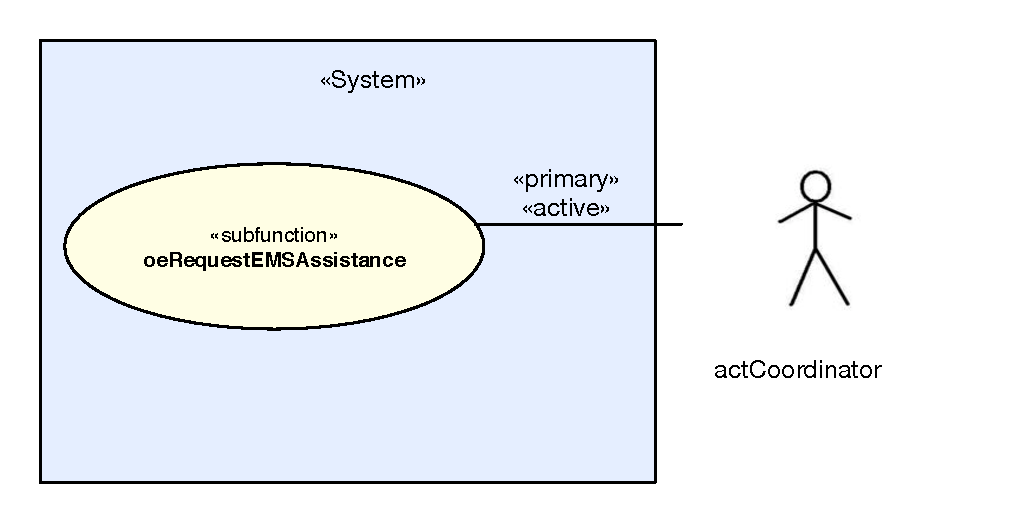
\includegraphics[width=180mm]{./images/oeRequestEMSAssistance.eps}
 \normalsize}
 \end{center}
 \caption[\msricrash Use Case Diagram:  oeRequestEMSAssistance Diagram]{\msricrash Use Case Diagram:  oeRequestEMSAssistance}
 \label{fig:icrash-RE-UCD- oeRequestEMSAssistance}
 \end{figure}
 \vspace{0.5cm}
